
Using the uniform erasure functions (or the erase-remove idiom) to delete items from the middle of a vector takes O(n) (linear) time. This is because elements must be shifted from the end of the vector to close the gap of the deleted items. If the order of items in the vector is not important, we can optimize this process to take O(1) (constant) time. Here's how.

\subsubsection{How to do it…}

This recipe takes advantage of the fact that removing an element from the end of a vector is quick and easy.

\begin{itemize}
\item 
Let's start by defining a function to print out a vector:

\begin{lstlisting}[style=styleCXX]
void printc(auto & r) {
	cout << format("size({}) ", r.size());
	for( auto & e : r ) cout << format("{} ", e);
	cout << '\n';
}
\end{lstlisting}

\item 
In our main() function we define a vector of int and print it using printc():

\begin{lstlisting}[style=styleCXX]
int main() {
	vector v{ 0, 1, 2, 3, 4, 5, 6, 7, 8, 9 };
	printc(v);
}
\end{lstlisting}

Output:

\begin{tcblisting}{commandshell={}}
size(10) 0 1 2 3 4 5 6 7 8 9
\end{tcblisting}

\item 
Now we'll write the function that will delete an element from the vector:

\begin{lstlisting}[style=styleCXX]
template<typename T>
void quick_delete(T& v, size_t idx) {
	if (idx < v.size()) {
		v[idx] = move(v.back());
		v.pop_back();
	}
}
\end{lstlisting}

The quick\_delete() function takes two arguments, a vector v and an index idx. We first check to make sure our index is within boundaries. Then we call the move() function from the <algorithms> header to move the last element of the vector to the position of our index. Finally, the v.pop\_back() function is called to shorten the vector from the back.

\item 
Let's also include a version of quick\_delete() for use with an iterator instead of an index.

\begin{lstlisting}[style=styleCXX]
template<typename T>
void quick_delete(T& v, typename T::iterator it) {
	if (it < v.end()) {
		*it = move(v.back());
		v.pop_back();
	}
}
\end{lstlisting}

This version of quick\_delete() operates from an iterator instead of an index.
Otherwise, it works the same as the indexed version.

\item 
Now we can call it from our main() function:

\begin{lstlisting}[style=styleCXX]
int main() {
	vector v{ 12, 196, 47, 38, 19 };
	printc(v);
	auto it = std::ranges::find(v, 47);
	quick_delete(v, it);
	printc(v);
	quick_delete(v, 1);
	printc(v);
}
\end{lstlisting}

And the output will look like this:

\begin{tcblisting}{commandshell={}}
size(5) 12 196 47 38 19
size(4) 12 196 19 38
size(3) 12 38 19
\end{tcblisting}

The first call to quick\_delete() uses an iterator from the std::ranges::find() algorithm. This deletes the value 47 from the vector. Notice the value from the back of the vector (19) takes its place. The second call to quick\_delete() uses an index (1) to delete the second element from the vector (196). Again, the value from the back of the vector takes its place.
\end{itemize}

\subsubsection{How it works…}

The quick\_delete() function uses a simple trick to delete elements from a vector quickly and efficiently. The element at the back of the vector is moved (not copied) into the position of the element to be deleted. The deleted element is discarded in the process.

Then, the pop\_back() function shortens the vector by one element from the end.
This takes advantage of the fact that deleting the element at the back of the vector is especially cheap. The pop\_back() function operates at constant complexity, as it only needs to change the end() iterator.

This diagram shows the state of the vector before and after the quick\_delete() operation:

\hspace*{\fill} \\ %插入空行
\begin{center}
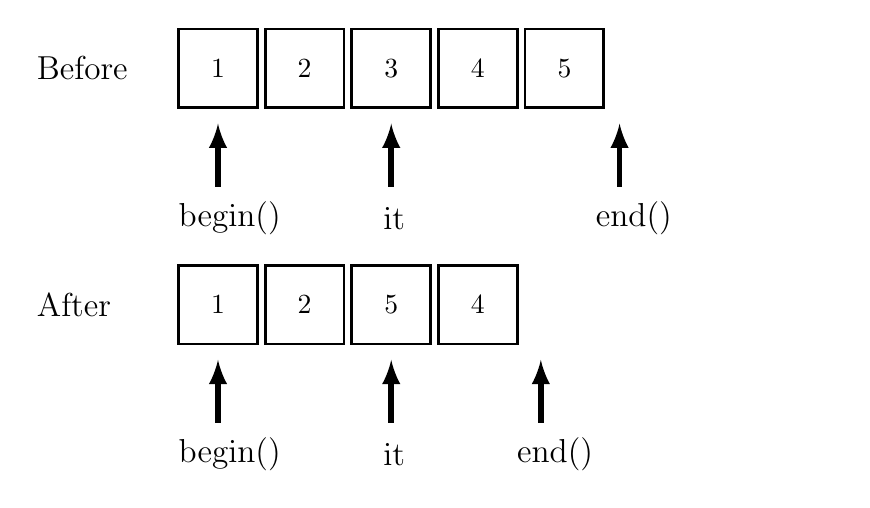
\begin{tikzpicture}
%before
\node[text width=3cm, font=\large] at (-0.3,0.5) {Before};

\foreach \x [evaluate=\x as \index using int(\x+1)] in {0,...,4} {
	\draw[line width=1pt] (1.1*\x,1) rectangle (1.1*\x+1,0) node[pos=.5] {\index};
}

\draw[line width=2pt][-latex] (0.5,-1.0) -- (0.5,-0.2);
\draw[line width=2pt][-latex] (2.7,-1.0) -- (2.7,-0.2);
\draw[line width=2pt][-latex] (5.6,-1.0) -- (5.6,-0.2);

\node[text width=3cm, font=\large] at (1.5,-1.4) {begin()};
\node[text width=3cm, font=\large] at (4.1,-1.4) {it};
\node[text width=3cm, font=\large] at (6.8,-1.4) {end()};

%after
\node[text width=3cm, font=\large] at (-0.3,-2.5) {After};
\draw[line width=1pt] (1.1*0,-3) rectangle (1.1*0+1,-2) node[pos=.5] {1};
\draw[line width=1pt] (1.1*1,-3) rectangle (1.1*1+1,-2) node[pos=.5] {2};
\draw[line width=1pt] (1.1*2,-3) rectangle (1.1*2+1,-2) node[pos=.5] {5};
\draw[line width=1pt] (1.1*3,-3) rectangle (1.1*3+1,-2) node[pos=.5] {4};

\draw[line width=2pt][-latex] (0.5,-4.0) -- (0.5,-3.2);
\draw[line width=2pt][-latex] (2.7,-4.0) -- (2.7,-3.2);
\draw[line width=2pt][-latex] (4.6,-4.0) -- (4.6,-3.2);

\node[text width=3cm, font=\large] at (1.5,-4.4) {begin()};
\node[text width=3cm, font=\large] at (4.1,-4.4) {it};
\node[text width=3cm, font=\large] at (5.8,-4.4) {end()};
\end{tikzpicture}

Figure 3.4 – Before and after quick\_delete()
\end{center}

The quick\_remove() operation simply moves the element from the back of the vector into the position of the iterator (it), then shortens the vector by one element. It's important to use std::move() instead of an assignment to move the element. The move operation is much faster than a copy-assignment, especially for large objects.

If you don't require ordered elements, this is an extremely efficient technique. It happens in constant (O(1)) time and without touching any other elements.









